\chapter{LL and LR algorithms}
\label{chap:ll_and_lr}
This chapter is interested in how to parse CFGs grammar. We will see two
algorithms : LL and LR. Note that, they are not generic algorithms for CFGs
parsing.

\section{Historical perspective}
    \begin{itemize}
        \item Chomsky's Hierarchy : mid-50s
        \item LL \& LR : formalized in mid/late 60
        \item Processors at this time where not very efficient
        \item $\mathcal{O}(n^3)$ was laughable, way to slow
    \end{itemize}

    Taking that into account, the choice to make efficient implementation (no
    backtracking / fancy data structure) that can only parse a part of CFGs was
    made. It is very practical, indeed we can show that programming language
    typically can be parse in $\mathcal{O}(n)$.
\section{LL}
    \theoremstyle{definition}
    \begin{definition}[LL]
        LL = Left-to-right Leftmost derivation. It always expand the left
        non-terminal first.
    \end{definition}
    It can parse a subset of CFGs :
        \begin{itemize}
            \item Choices: use k tokens of lookahead to decide (never backtrack)
            \item Nowadays we consider it as a worse PEG
            \item If the grammar is accepted by LL, it guarantees
            $\mathcal{O}(n)$, can be implemented based on table-based lookup
        \end{itemize}
    \subsection{Properties}
        \begin{itemize}
            \item Top down recursive descent algorithm as PEG (but only one
            choice alternative taken, depends on lookahead lookup)
            \item No left recursion allowed
            \item Like PEG : unambiguous
            \item No language hiding (\[A ::= a* a\] is not a valid language in LL)
            \item Less expressive than CFG or PEG (even than LR)
        \end{itemize}

        \theoremstyle{definition}
        \begin{definition}[LL Grammar]
            Grammar for which we can generate an LL parser (no FIRST/FIRST or
            FIRST/FOLLOW conflicts)
        \end{definition}
        \theoremstyle{definition}
        \begin{definition}[LL Language]
            A language that has a LL grammar (may have multiple grammars
            including non-LL ones.)
        \end{definition}
        \subsubsection{LL Conflicts}
            \paragraph{FIRST/FIRST conflit}
                \begin{itemize}
                    \item Choices starting with the same k tokens
                    \item $A ::= ab | ac (k=1)$
                \end{itemize}
            \paragraph{FIRST/FOLLOW conflit}
                \begin{itemize}
                    \item Choice can start or (if it is nullable) be followed by
                    the same k tokens ($S ::= X Y ; X ::= \epsilon | a; Y ::= a | b$)
                \end{itemize}

                We can avoid FIRST/FIRST with left-factoring (factor out the
                common part at the start of two choice alternatives)
                \begin{figure}[H]
                     \centering
                     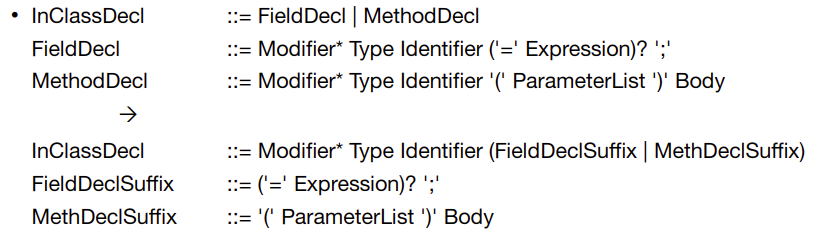
\includegraphics[scale=0.4]{LL_Conflict_avoid.png}
                     \caption{Left-factoring example}
                     \label{fig:left-factoring}
                \end{figure}
                
                In the previous figure, the three first line are not LL as the
                two last starts with the same prefix. The 3 last lines are LL
                because the suffix has been extracted, so the both use the same
                rule with a suffix choice instead of two rules.

                Note that it is not great for plain syntax tree, also makes the
                AST a bit more difficult to build. However it is also useful for
                PEG performance (we avoid parsing the same prefix many times).
    \subsection{LL(1) vs Regular Expression}
        As both of them use a single symbol we could ask why are they not the same.
        \begin{itemize}
            \item LL can handle central recursion
            \item Regular grammars are parser with $\mathcal{O}(1)$ space (current state)
            \item LL(1) implemented by top-down recursive descent uses
            $\mathcal{O}(n)$ space: the function call stack (can be use to
            recurse) 
        \end{itemize}
\section{LR}